% -------------------------------------------------------
% Results
% -------------------------------------------------------

\section{Results}

Meta-analyses of eye movements are relatively rare, potentially because of methodological challenges in combining effect sizes from different eye-tracking studies. Two main challenges are how to handle measurement validity across eye-tracker types and how to compare different eye movement dependent variables. To handle these issues, we developed correction procedures integrated in a psychometric meta-analysis \citep{hunter2004a}, which allow us to quantify the interference of measurement validity or multiple metrics. The measurement validity issue stems from differences in the accuracy and precision of eye-tracking equipment \citep{holmqvist2015a}, which can affect the data quality and bias effect sizes \citep{orquin2016a}. We developed a correction method that relies on an empirical estimate of the relationship between eye-tracker characteristics and observed effect sizes (see \textit{Method}; Figure~\ref{fig:ET_accuracy_effectsize}; Table~\ref{tab:eyetracker_specifications}). Most metrics are based on fixations -- defined as maintaining the gaze at a single location or area of interest (AOI), such as fixation count, fixation likelihood, total dwell time, and so on. This leads to a potential issue with comparing effect sizes reported with different dependent variables. We developed a correction method that makes the dependent variables comparable, where we empirically estimate correction factors based on a subset of studies in our sample that report multiple dependent variables (see \textit{Method}; Figure~\ref{fig:metric_correction}; Table~\ref{tab:metric_correction}). This method allowed us to transform all effect sizes to a single metric; we decided for fixation count, which was used in all meta-analyses. 

To understand the context in which the studies were conducted, we coded participant sample information -- age, gender, ethnicity, and country -- across visual and cognitive factors (Table~\ref{tab:sampleTable} in the Appendix). Generally, participant samples include a roughly even split of men and women in many cases with a mean age above 30. The studies are collected in a wide range of countries, but are with few exceptions restricted to white participants. 

In what follows, we first analyze the group of visual factors and then the group of cognitive factors. We perform a meta-analysis on each individual factor  separately. We next perform a small moderator analysis and finish with an analysis of publication bias in all the meta-analyses.


\subsection{Almost all visual factors have substantial effect sizes}

We focused on four major groups of visual factors -- salience, position, surface size, and set size (see \textit{Method} for coding procedure). The summary effects of the visual factors on attention during decision making show that the factors range from small to medium effect sizes (see Table~\ref{tab:main_results} and Figure~\ref{fig:forest_plots_visual}). Since the publication bias analyses suggest the presence of bias (see \textit{Publication bias} section below), we conducted a sensitivity analysis that indicates the possible extent of bias in individual factors. The Top10 sensitivity analysis (see \textit{Method} for details) suggests large upward adjustment for three factors -- salience, surface size, and center position -- resulting in medium to large effect sizes (Table~\ref{tab:main_results}; results in parentheses). For set size the Top10 analysis suggests no change in effect size, while for left vs. right position it suggests large downward correction to a near null effect. While the left vs. right position does not seem to have an effect on fixation count, we cannot exclude effects on temporal dynamics. For instance, decision makers may be more likely to begin with the left option and then move right \citep{fiedler2012}, which could lead to primacy effects on choice. Overall, the Top10 analysis suggests that there is some publication bias in the visual factors. Inspecting the effect sizes, it is interesting that salience, which so far has taken the center stage in vision science, has smaller summary effect than some of the other visual factors. The largest effects are those of center position, $r=.43$, and surface size, $r=.35$, which are on par with cognitive factors, which range between $r = .35$ and $r = .59$. If considering the Top10 analysis results, then visual factors are substantially larger than cognitive factors. While it is possible to eliminate the effects of, for instance, center position and surface size in laboratory studies, this is not true for natural environments. In natural environments it is reasonable to expect that multiple, and most likely all, visual factors influence eye movements at the same time. Not only do the effects of the largest visual factors exceed the largest cognitive factors when comparing one by one, but considering their joint effect we believe it is reasonable to conclude that visual factors play a larger role than cognitive factors in determining visual attention in decision making. 


% latex table generated in R 3.6.3 by xtable 1.8-4 package
% Sat Jun 20 12:32:29 2020
\begin{table}[ht]
\centering
\caption{Main results of the meta-analysis, divided into visual and cognitive factor groups, and individual factors within them. The most important values are the corrected effect size estimate, $\rho$, and the associated heterogeneity, $I^2$. Results of trim and fill analysis are in the parentesis.} 
\label{tab:main_results}
\begingroup\small
\begin{tabular}{lp{0.03\linewidth}p{0.05\linewidth}p{0.07\linewidth}p{0.07\linewidth}p{0.07\linewidth}p{0.07\linewidth}p{0.07\linewidth}p{0.07\linewidth}p{0.07\linewidth}}
  \hline
Group & $k$ & $N$ & $\rho$ & SE & $Z$ & $p$ & $\textrm{CI}_{95}$ LL & $\textrm{CI}_{95}$ UL & $I^2$ \\ 
  \hline
\textbf{Visual factors} &  &  &  &  &  &  &  &  &  \\ 
  Salience & 9 (1) & 530 & 0.11 (0.11) & 0.066 (0.121) & 1.659 (0.911) & 0.097 (0.362) & -0.02 (-0.127) & 0.24 (0.335) & 0 \\ 
  Surface size & 6 (0) & 740 & 0.396 (0.508) & 0.108 (0.188) & 3.682 (2.986) & 0 (0.003) & 0.185 (0.19) & 0.607 (0.73) & 55.31 \\ 
  Left vs right position & 3 (0) & 415 & 0.316 (0.485) & 0.213 (0.32) & 1.484 (1.652) & 0.138 (0.099) & -0.101 (-0.098) & 0.733 (0.82) & 46.04 \\ 
  Center position & 11 (0) & 912 & 0.434 (0.622) & 0.086 (0.209) & 5.065 (3.48) & 0 (0.001) & 0.266 (0.308) & 0.602 (0.814) & 49.92 \\ 
  Set size & 10 (0) & 610 & 0.29 (0.348) & 0.094 (0.126) & 3.095 (2.891) & 0.002 (0.004) & 0.106 (0.116) & 0.473 (0.544) & 55.06 \\ 
  \textbf{Cognitive factors} &  &  &  &  &  &  &  &  &  \\ 
  Task instructions & 26 (0) & 1990 & 0.419 (0.516) & 0.059 (0.084) & 7.146 (6.789) & 0 (0) & 0.304 (0.385) & 0.534 (0.626) & 43.75 \\ 
  Preferential viewing & 21 (0) & 2014 & 0.476 (0.75) & 0.086 (0.171) & 5.544 (5.677) & 0 (0) & 0.308 (0.563) & 0.645 (0.864) & 79.87 \\ 
  Choice bias & 18 (6) & 625 & 0.695 (0.949) & 0.086 (0.263) & 8.088 (6.929) & 0 (0) & 0.527 (0.863) & 0.864 (0.981) & 67.51 \\ 
   \hline 
 \multicolumn{10}{p{0.9\textwidth}}{\scriptsize{\textit{Note.} $k$ = number of studies (for trim and fill analysis number of imputed studies); $N$ = number of participants; $\rho$ = unattenuated effect size estimate, SE = standard error of estimate; $Z$ = Z statistic; $p$ = significance level; $\textrm{CI}_{95}$ LL = lower limit of the 95\% confidence interval; $\textrm{CI}_{95}$ UL = upper limit of the 95\% confidence interval, $I^2$ = within-group heterogeneity.}} 
\end{tabular}
\endgroup
\end{table}



\begin{figure}[!h]
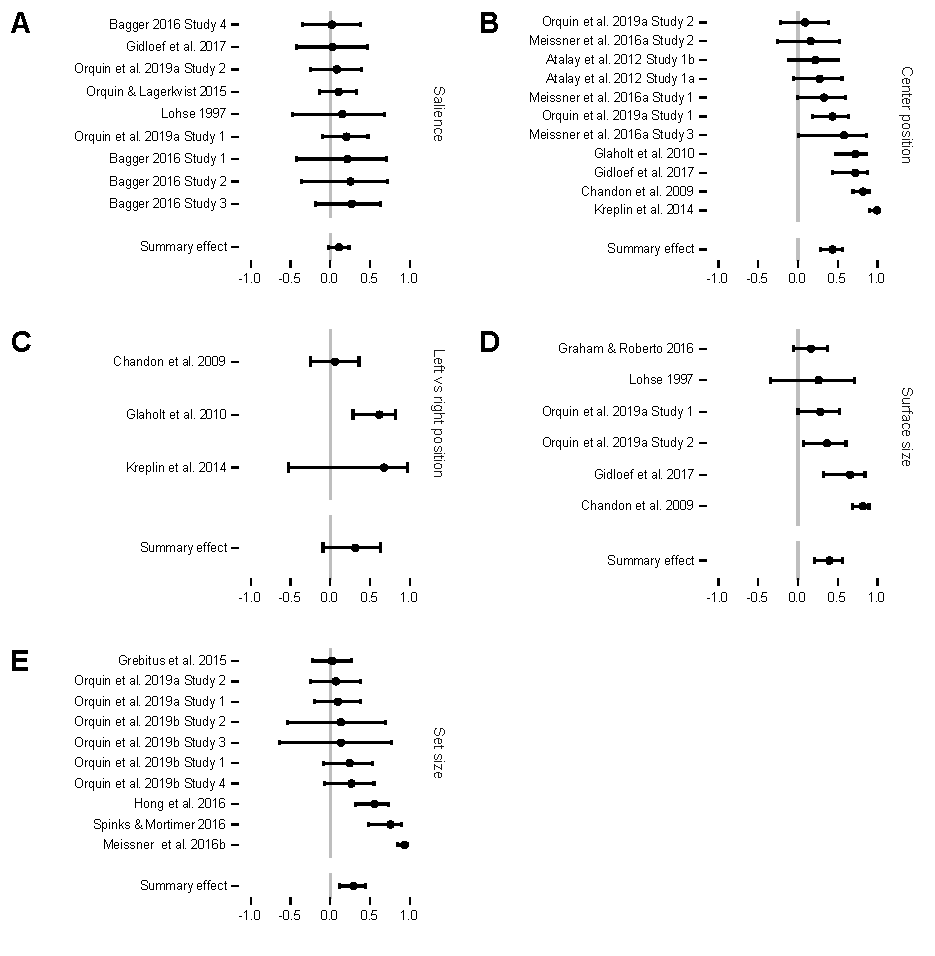
\includegraphics{forest_plots_visual}
\centering
\caption{Effect sizes of the visual factors are moderate, except for salience and left vs. right position, which have small effect sizes, if any. Forest plots show the unattenuated effect size correlations for each study in a group, as well as average effect across the group. Forest plot in (A) shows the effect sizes for salience factor, in (B) for center position, in (C) for left vs. right position, in  (D) for surface size, and in (E) for set size factor. Error bars represent the 95\% confidence interval around the mean.}
\label{fig:forest_plots_visual}
\end{figure}


\subsection{Cognitive factors have effect sizes similar in magnitude to visual factors}

Previous research has identified a wide range of cognitive factors that influence attention, such as goals, task instructions, and preferences \citep[for a review see][]{orquin2013a}. Here, we divided cognitive control factors into three groups: task instruction, preferential viewing, and choice-gaze effect. In studies on task instructions, participants receive instructions concerning a specific decision goal, and with that, what is it relevant to gaze at. For instance, the participants may be instructed on the validity of stimulus attributes \citep{krefeld-schwalb2019a}, or infer the level of validity themselves \citep{bialkova2014a}. In preferential viewing studies, the relevance should be equal to the subjective preferences. For example, some alternatives have higher subjective values than others \citep{kim2012a}. Because of this qualitative difference between the two domains, we treated studies on task instructions and preferential viewing separately. 
Inspecting the effect sizes reveals that the summary effects in the two types of studies are moderate and similar in magnitude (see Table~\ref{tab:main_results} and Figure~\ref{fig:forest_plots_cognitive}). Using a Wald test, we find that effect sizes of task instructions and preferential viewing are unlikely to differ, $z=-0.033$, $p=0.399$. 
The test suggests that it makes no difference to eye movements whether the relevance of information is defined according to an externally specified goal or according to preferences. Note, however, that the two effect sizes differ more when comparing the effect sizes from the Top10 analysis, which suggests downward adjustments, with larger adjustment for task instructions (Table~\ref{tab:main_results}; results in parentheses).

Choice-gaze effect refers to an effect in attention whereby decision makers spend more time gazing at the eventually chosen alternative. This effect, originally introduced by Shimojo and colleagues \citep{shimojo2003a} as a ``gaze-cascade'' effect, is well-established in the literature, prompting us to study it as a separate factor. This factor consists of studies reporting the difference in eye movements between the chosen alternative and all other (not chosen) alternatives. We find that choice-gaze effect has a large effect on eye movements, $r=.59$. However, the Top10 analysis suggests a large downward adjustment, to a small effect, $r=.26$.


\begin{figure}[!h]
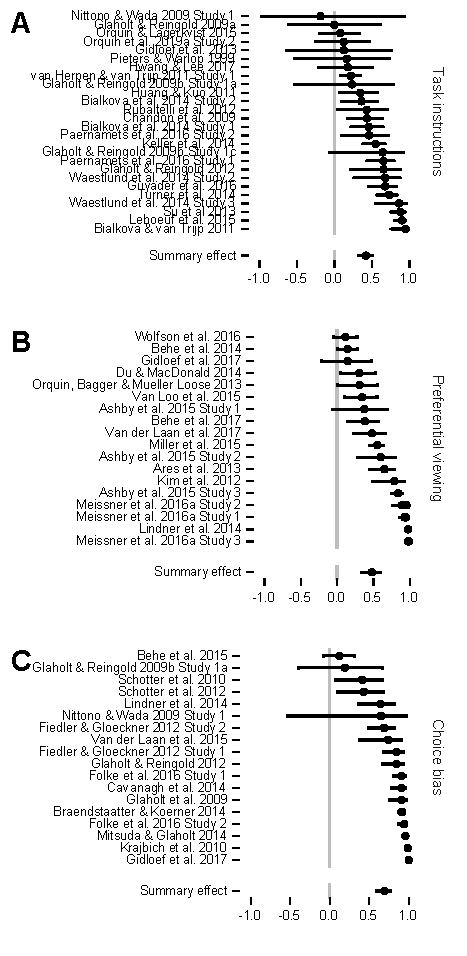
\includegraphics{forest_plots_cognitive}
\centering
\caption{Effect sizes of the three cognitive factors are moderate to large. Forest plots show the unattenuated effect size correlations for each study in a group, as well as average effect across the group. Forest plot in (A) shows the effect sizes for task instructions factor, in (B) for preferential viewing, and in (C) for the choice-gaze effect factor. Error bars represent the 95\% confidence interval around the mean.}
\label{fig:forest_plots_cognitive}
\end{figure}


\subsection{Alternative vs. attribute moderator is significant only for the set size factor}

Alternatives that participants in judgment and decision making studies choose between can often be decomposed into constituent elements, commonly called attributes, cues, or features \citep{payne1988,tversky1972elimination,stojic2020s,gigerenzer1996reasoning,schulz2018putting,hogarth2007heuristic}. For example, in classical lottery tasks \citep{tversky1979}, the probabilities and values of an alternative can be viewed as attributes. Or, in multi-cue judgment tasks, alternatives are more explicitly composed of cues -- in the German city size task, for example, these would be university, major football team, main city, and so on \citep{gigerenzer1996reasoning}. This has consequences for both modelling of decision processes and units of analysis. Consequently, some studies in our sample focused on attention effects at either alternative or attribute level, or both. This was in particular the case for studies involving set size, task instructions, and preferential viewing factors. Since the alternative vs. attribute dimension might be an important moderator in these groups, we decomposed them further with regards to the effect of alternatives vs. attributes (Table~\ref{tab:mod_results} and Figure~\ref{fig:forest_plots_altatt}). Moderator analyses show support for the alternative vs. attribute moderator across set size, $Q_M(1)=4.765$, $p=0.029$\unskip, but no support for preferential viewing, $Q_M(1)=4.312$, $p=0.038$\unskip, or for task instructions, $t=-0.213$, $p=0.835$\unskip. It is worth noting that effect sizes are consistently larger when operationalized at the level of alternatives compared to attributes (Table~\ref{tab:mod_results} and Figure~\ref{fig:forest_plots_altatt}). 

We also performed a moderator analysis for the choice-gaze effect factor, to assess whether the effect is driven by preferential viewing as proposed by \cite{shimojo2003a}. We compare studies with preferential vs. inferential choice tasks and find no support for moderation by decision type, $Q_M(1)=0.057$, $p=0.811$\unskip, and therefore only report results for the main group. 


% -------------------------------------------------------
% Publication bias
% -------------------------------------------------------

\subsection{Publication bias exists, but mainly affects cognitive factors}

We assessed potential publication bias by first performing a precision-effect test \citep[PET][]{stanley2014}, which regresses individual study effect sizes on study standard deviations weighted by the study precision, controlling for the eye-tracker accuracy in addition (see \textit{Method} for details). It is not recommended to use the test in case of small samples (for example, less than 10 studies \citep{vanaert2019}), and we therefore used it on the complete data set. Because many articles report more than one effect size we computed robust variance estimates of all model coefficients based on a sandwich-type estimator. The PET shows a significant effect of standard deviation of the effect size, $\beta=2.16$, $SE=0.63$, $p=0.01$\unskip, suggesting the presence of publication bias (see \textit{Appendix} Table \ref{tab:PET-PEESE} for full regression results). Given the significant PET, we then performed the precision-effect estimate with standard errors test (PEESE). The PEESE differs only in using the study variance instead of the standard deviation. The intercept in the PEESE is normally used as the publication bias corrected estimate, $\beta=0.23$, $SE=0.1$, $p=0.17$ (see \textit{Appendix} Table \ref{tab:PET-PEESE} for full regression results). The bias corrected estimate in the PEESE test is, in our case, not very informative by itself since it groups all independent variables into one estimate. However, by comparing the PEESE intercept to that obtained from an intercept only regression, % latex table generated in R 3.5.2 by xtable 1.8-4 package
% Tue Dec  1 11:40:08 2020
\begin{table}[ht]
\centering
\caption{Fixed effects analysis of complete data} 
\label{tab:FE}
\begingroup\small
\begin{tabular}{llccc}
  \hline
Parameter & Estimate & SE & t & p \\ 
  \hline
Intercept & 0.29 & 0.03 & 10.82 & 0.00 \\ 
  \end{tabular}
\endgroup
\end{table}
\unskip, we can get an impression of the degree of effect size overestimation due to publication bias. This comparison suggests that publication bias leads to an overestimation factor of $1.278$\unskip.

We performed an additional analysis of publication bias because of the above-mentioned limitations of the PET-PEESE test. It has been shown that studies which receive public grants are more likely to be published \citep{canestaro2017}, and we therefore expected that acknowledging a public grant in the article may be associated with smaller effect sizes. We used a random effects model with robust variance estimation and public grant as moderator (see \textit{Method}). We find that although public grants are associated with smaller effect sizes, the moderator does not have a significant effect, $Q_M(1)=0.12$, $p=0.73$\unskip. Comparing public vs. non-public funded research we derived an overestimation factor of $1.392$\unskip, which is nevertheless higher than the estimate derived from the PET-PEESE analysis.

The PET-PEESE and public grant analyses are based on very different premises, but they both indicate the presence of publication bias. We therefore proceeded with a Top10 analysis, an additional sensitivity analysis at the level of each independent variable (see \textit{Method}). The Top10 analysis resulted in an upward adjustment of the average effect size for several visual factors, downward adjustment for all cognitive factors and the visual factor left vs. right position. The corrected effect sizes in Table~\ref{tab:main_results} (in parentheses) provide a more conservative estimate of the true population effects, but are also subject to some uncertainty because of a relatively small number of studies in the visual factor groups. Comparing the Top10 with the uncorrected estimates suggests an overestimation factor of $1.388$\unskip, which is close to the overestimation factors from the PET-PEESE and the public grant analysis.

The three analyses suggest an overestimation factor somewhere in the range of $1.278$ to $1.388$\unskip. While any factor above 1 is undesirable, it is worth noting that it is far below the factor of 2.59 suggested by \cite{kvarven2020} who compared 15 pairs of meta-analysis estimates with estimates from many-lab replication studies. In addition to these analyses, we plotted the Fisher transformed correlation coefficients of each study by its respective standard error (so-called funnel plots; Figure~\ref{fig:funnel_plots} for main results, and Figure~\ref{fig:funnel_plots_altatt} for moderator analyses). The symmetry of the funnel plots provides a qualitative picture of publication bias since we expect that studies with smaller sample sizes and hence higher standard errors yield more variable effect sizes, the smallest of which are less likely to be published, leading to an asymmetric funnel plot. Funnel plots are generally rather difficult to interpret, and in our case it is almost impossible to draw any conclusion for visual factors, given the smaller number of studies on which they are based.


% -------------------------------------------------------
% Descriptive EM analysis
% -------------------------------------------------------


\subsection{Projecting effect sizes to original measurement units reveals substantial effects in absolute sense}

To better understand the results of the meta-analysis we extract for each effect size the corresponding descriptive eye movement data whenever the included study reports this information (see \textit{Method}). For example, a study would report a fixation count (or likelihood or dwell time) for high vs. low salience conditions. We extracted the descriptive eye movement data at the unit of a single AOI, for example, corresponding to the fixation count for a single attribute level or for a single alternative if the AOIs are defined at this level. A total of $34$\unskip articles report descriptive eye movement data, resulting in $93$\unskip corresponding pairs of effect sizes and descriptive eye movement data, with some studies reporting results for more than one dependent variable. In total, there are $39$\unskip studies reporting fixation likelihood, $28$\unskip reporting fixation count, and $35$\unskip reporting total dwell time.


\begin{figure}[!h]
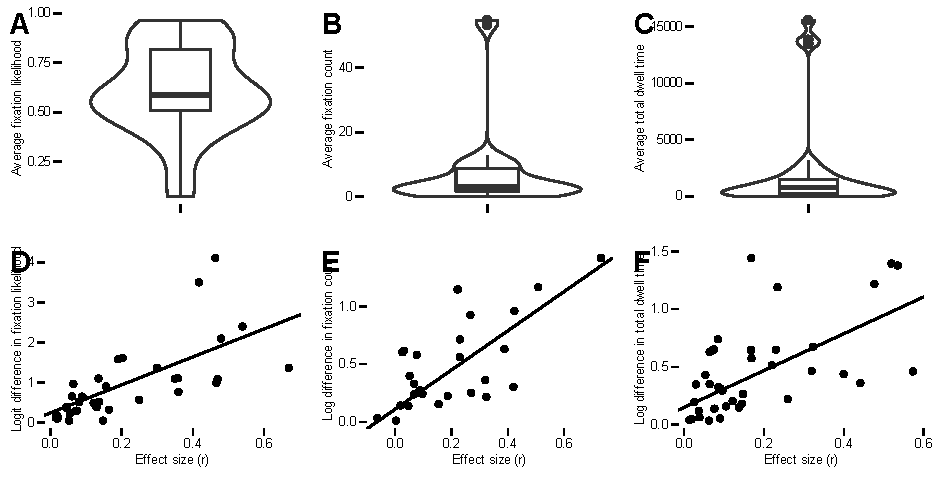
\includegraphics{figs/EMtoES.pdf}
\centering
\caption{Descriptive eye movement data provides insight into the attention behavior of an average participant and how effect sizes translate into the original measures on which they were based. Distribution plots illustrate the fixation likelihood (A), the average fixation count (B), and the average total dwell time (C) across studies. We illustrate the linear relationship between the effect size correlation and the descriptive eye movement data by logit transforming differences in fixation likelihood (D), log transforming fixation count (E), and log transforming total dwell time (F). Lines are based on intercepts and slopes from linear mixed model fits (see main text and \textit{Method} for details).}
\label{fig:em_figure}
\end{figure}


From averaged eye movement measures we see that the average for fixation likelihood is $M=0.614$, $SD=0.233$\unskip, for fixation count $M=7.773$, $SD=13.559$\unskip, and total dwell time $M=2253.505$, $SD=4258.481$\unskip. From the distribution plots it is clear that there is a lot of variance in fixation likelihood across studies (Figure~\ref{fig:em_figure}). In some studies participants fixate nearly all AOIs, but there is also a large number of studies in which participants fixate half or less of the AOIs. The main use of the descriptive eye movement data, however, was to provide intuitions about the synthesized effect sizes. To this end, we transformed the synthesized effect size for each independent variable into its corresponding effect on fixation likelihood, fixation count, and total dwell time (see \textit{Method} for details). We achieved this transformation by regressing descriptive measures (appropriately transformed) on effect size correlations, using a linear mixed model with a random intercept, grouped by article to account for correlated errors. For fixation likelihood (logit difference between conditions), the model intercept is not significantly different from zero, whereas the slope is, $\beta_{0}=0.24$, $SE=0.21$, $p=0.25$, $\beta_{1}=3.49$, $SE=0.5$, $p< 0.001$\unskip. Figure \ref{fig:em_figure} panel (D) illustrates the relationship between the transformed statistic and effect size correlations, with an increasing variance as effect sizes become larger. For fixation count (log difference between conditions), the model shows a similar pattern where the intercept is not significantly different from zero, while the slope is, $\beta_{0}=0.05$, $SE=0.1$, $p=0.64$, $\beta_{1}=1.83$, $SE=0.32$, $p< 0.001$\unskip, as illustrated in Figure~\ref{fig:em_figure} panel (E). The model for total dwell time (log difference between conditions) reveals the same pattern, $\beta_{0}=0.13$, $SE=0.09$, $p=0.15$, $\beta_{1}=1.71$, $SE=0.35$, $p< 0.001$\unskip, as illustrated in Figure~\ref{fig:em_figure} panel (F). Overall, all three measures strongly correlate with the (transformed) effect sizes, giving us confidence for converting effect sizes into original measures using the fitted models. More specifically, for each independent variable we computed the expected increase in descriptive eye movement measures based on the effect size, for a study with an average descriptive measure (see \textit{Method} for details). Combining the estimates from these operations we could finally compare the effect sizes for each independent variable in terms of the equivalent effect on fixation likelihood, fixation count, and total dwell time for an average study (see Table~\ref{tab:em_results}). The table reveals surprisingly large effects on eye movements when expressing effect size correlations in raw eye movement metrics. Even the smallest effect observed for salience, $\rho = .13$, leads to an increase in fixation likelihood from an average of $61\%$ to $76\%$. Using a central location increases fixation likelihood to $91\%$. For fixation count the numbers are equally surprising. From an average fixation count of $7.8$, increasing salience can add three more fixations to a piece of information, while using a central location can add nearly ten more fixations. For the purpose of policy interventions aiming to capture decision maker attention, these numbers are beyond all our expectations.

% latex table generated in R 3.5.2 by xtable 1.8-4 package
% Fri Nov 27 09:37:38 2020
\begin{table}[ht]
\centering
\caption{Main effects expressed as absolute changes in the fixation likelihood, fixation count, and total dwell time.} 
\label{tab:em_results}
\begingroup\small
\begin{tabular}{p{3.7cm}p{1.2cm}p{1.3cm}p{1.3cm}p{1.3cm}p{1.3cm}p{1.6cm}p{1.6cm}}
  \hline
Group & \rho & FL L & FL U & FC L & FC U & TDT L & TDT U \\ 
  \hline
Salience & 0.13 & 0.61 & 0.76 & 7.80 & 10.92 & 2196.59 & 3081.09 \\ 
  Surface size & 0.35 & 0.61 & 0.89 & 7.80 & 15.28 & 2196.59 & 3954.68 \\ 
  Left vs right position & 0.24 & 0.61 & 0.83 & 7.80 & 12.92 & 2196.59 & 3490.66 \\ 
  Center position & 0.43 & 0.61 & 0.91 & 7.80 & 17.26 & 2196.59 & 4330.43 \\ 
  Set size & 0.24 & 0.61 & 0.83 & 7.80 & 12.92 & 2196.59 & 3490.66 \\ 
  Task instructions & 0.35 & 0.61 & 0.89 & 7.80 & 15.28 & 2196.59 & 3954.68 \\ 
  Preferential viewing & 0.36 & 0.61 & 0.89 & 7.80 & 15.51 & 2196.59 & 3999.80 \\ 
  Choice bias & 0.59 & 0.61 & 0.95 & 7.80 & 22.03 & 2196.59 & 5192.44 \\ 
   \hline 
 \multicolumn{8}{p{0.95\textwidth}}{\scriptsize{\textit{Note.} 
                   FL L = lower fixation likelihood,
                   FL U = upper fixation likelihood,
                   FC L = lower fixation count,
                   FC U = upper fixation count,
                   TDT L = lower total dwell time,
                   TDT U = upper total dwell time}} 
\end{tabular}
\endgroup
\end{table}

